\chapter{FUNCTIONAL VERIFICATION}
\label{chap:func_verif}

\section{INTRODUCTION}
Functional verification involves determining whether or not a logic design matches a specification of its intended behavior. A testbench is built to functionally verify the design by providing meaningful scenarios to check that given certain input, the design performs to specification. In simulation, the testbench wraps around the Design Under Test (DUT), just as a hardware tester connects to a physical chip, as shown in ~\figurename~{\ref{fig:testbench.png}}.
\vspace{10pt}
\begin{figure}[h!]
\centering
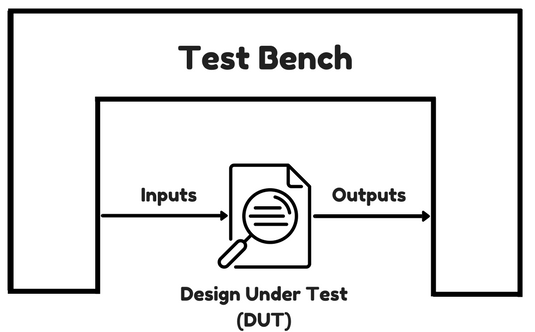
\includegraphics[scale=0.6]{./figures/testbench.png}
\caption{Testbench-Design Environment}
\label{fig:testbench.png}
\end{figure}

\section{LAYERED TESTBENCH}
Layered testbench is a key concept for any modern verification methodology. This kind of testbench makes the task easier by dividing the code into smaller pieces that can be developed separately.
\vspace{10pt}
\begin{figure}[h!]
\centering
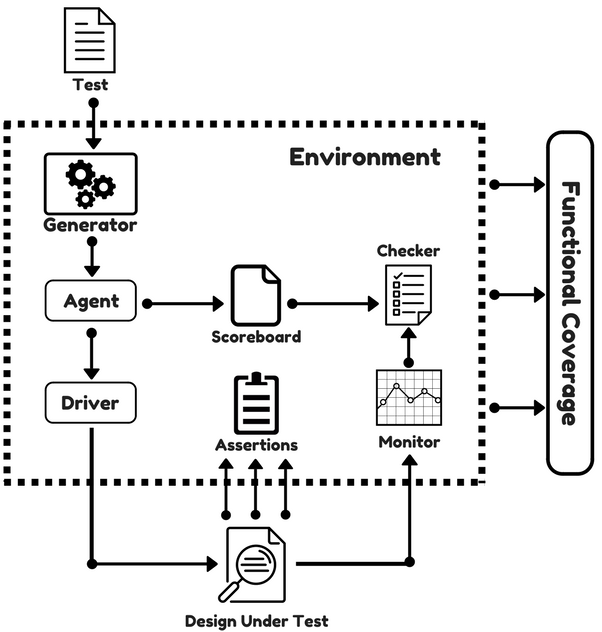
\includegraphics[scale=0.9]{./figures/layered_testbench.png}
\caption{Layered Testbench}
\label{fig:layered_testbench.png}
\end{figure}

\subsection{SIGNAL LAYER}
Signal layer is at the bottom which contains the DUT and the signals that connect it to the testbench.

\subsection{COMMAND LAYER}
The next higher level is the command layer. The DUT’s inputs are driven by the driver that runs single commands, such as bus read or write. The DUT’s output drives the monitor that takes signal transitions and groups them together into commands. Assertions also cross the command/signal layer, as they look at individual signals but look for changes across an entire command.
\paragraph{Driver:} The drivers translate the operations produced by the generator into the actual inputs for the design under verification. Generators create inputs at a high level of abstraction namely, as transactions like read write operation. The drivers convert this input into actual design inputs, as defined in the specification of the designs interface. If the generator generates read operation, then read task is called, in that, the DUT input pin "read-write" is asserted.
\paragraph{Monitor:} Monitor reports the protocol violation and identifies all the transactions. Monitors are two types, Passive and active. Passive monitors do not drive any signals. Active monitors can drive the DUT signals. Sometimes this is also refered as receiver. Monitor converts the state of the design and its outputs to a transaction abstraction level so it can be stored in scoreboard database to be checked later on. Monitor converts the pin level activities in to high level.
\paragraph{Assertions:} Assertions are used to check time based protocols, also known as temporal checks. Assertions are a necessary compliment to transaction based testing as they describe the pin level, cycle by cycle, protocols of the design. Assertions are also used for functional coverage. 

\subsection{FUNCTIONAL LAYER}
Functional layer feeds down into the command layer. The agent block (also called the transactor) receives higher-level transactions such as DMA read or write and breaks them into individual commands. These commands are also sent to the scoreboard that predicts the results of the transaction. The checker compares the commands from the monitor with those
in the scoreboard.
\paragraph{Transactor:} Transactor does the high level operations like burst-operations into individual commands, sub-layer protocol in layered protocol like PciExpress Transaction layer over PciExpress Data Link Layer, TCP/IP over Ethernet etc. It also handles the DUT configuration operations. This layer also provides necessary information to coverage model about the stimulus generated. Stimulus generated in generator is high level like Packet is with good crc, length is 5 and da is 8~Rh0. This high level stimulus is converted into low level data using packing. This low level data is just a array of bits or bytes. Packing is an operation in which the high level stimulus values scalars, strings, array elements and struct are concatenated in the specified manner.
\paragraph{Scoreboard:} Scoreboard is sometimes referred as tracker. Scoreboard stores the expected DUT output. Scoreboard in Verilog tends to be cumbersome, rigid, and may use up much memory due to the lack of dynamic data types and memory allocation. Dynamic data types and Dynamic memory allocation makes it much easier to write a scoreboard in SystemVerilog. The stimulus generator generated the random vectors and is sent to the DUT using drivers. These stimuli are stored in scoreboard until the output comes out of the DUT.
\paragraph{Checker:} The monitor only monitors the interface protocol. It doesn't check the whether the data is same as expected data or not, as interface has nothing to do with the date. Checker converts the low level data to high level data and validated the data. This operation of converting low level data to high level data is called Unpacking which is reverse of packing operation. For example, if data is collected from all the commands of the burst operation and then the data is converted in to raw data , and all the sub fields information are extracted from the data and compared against the expected values. The comparison state is sent to scoreboard. 

\subsection{SCENARIO LAYER}
The generator in the scenario layer drives the functional layer. It generates input vectors that are used to search for anomalies that exist between the intent (specifications) and the implementation.
\paragraph{Generator:} The generator component generates stimulus which are sent to DUT by driver. Stimulus generation is modeled to generate the stimulus based on the specification. For simple memory stimulus generator generates read, write operations, address and data to be stored in the address if its write operation. Scenarios like generate alternate read/write operations are specified in scenario generator. SystemVerilog provided construct to control the random generation distribution and order. Constraints defined in stimulus are combinatioural in nature where as constraints defined in stimulus generators are sequential in nature. 

\subsection{TEST LAYER}
The top-most layer of testbench is the test layer. The test contains the constraints to create the stimulus. Tests can communicate with all the TestBench components.

\subsection{FUNCTIONAL COVERAGE}
Functional coverage measures the progress of all tests in fulfilling the verification plan requirements. The functional coverage code changes through the project as the various criteria complete. This code is constantly being modified, and thus it is not part of the environment.
